\section{Experiment 1 - Validation}
\label{sec:phase1}
For the first experiment the single objective functions are validated by using them as fitness function in the Evo-RoleMiner. A basic setup is chosen seen in Table \ref{tab:setup1}. The experiments are based on the small synthetic dataset 1. The number for individuals and generation is chosen relatively low since it is not aim to find a solution but rather to confirm the implementation and to analyse the single objectives in relation to each other. \\
\begin{table}[H]
    \centering
    \begin{tabular}{|l|l|}
        \hline
        \rowcolor{gray!25} 
        \textbf{Parameter}              & \textbf{Value}    \\ \hline
        Generations                     & 100              \\ \hline
        Population                      & 100              \\ \hline
        CXPB                            & 0.25              \\ \hline
        MUTPB                           & 0.25              \\ \hline
        MUTPB-Type1: Add role           & 0.25              \\ \hline
        MUTPB-Type2: Add User           & 0.25              \\ \hline
        MUTPB-Type3: Add Permission     & 0.25              \\ \hline
        MUTPB-Type4: Remove Role        & 0.25              \\ \hline
        MUTPB-Type5: Remove User        & 0.25              \\ \hline
        MUTPB-Type6: Remove Permission  & 0.25              \\ \hline
        Tournament size                 & 2                 \\ \hline
        Local optimization              & True              \\ \hline
    \end{tabular}
    \caption{EXPERIMENT 1 setup}
    \label{tab:setup1}
\end{table}
For the single objective "Minimizing Confidentiality" it is expected that the individuals (role models) violate confidentiality compared to the original access configuration $UPA$ less over time. The results in Figure \ref{fig:exp1conf} are confirming this and also show that individuals have less roles over time. This can be explained by that a lower count of roles probably result in less user-role- and role-permission assignments, which on the other hand lowers the probability of violating confidentiality. At the same time less user-role- and role-permission assignments let the probability for availability violations rise, which can be also seen in Figure \ref{fig:exp1conf}.

An opposite impact can be seen when single objective "Minimizing Availability" is used as fitness function (see Figure \ref{fig:exp1accs}). In the first generations the availability violations quickly achieve the goal of zero. During the same generations the role count, user-role- and role-permission assignments are rising. It is more likely that every user gets his permission (given in the original UPA-Matrix), if the amount of roles, user-role- and role-permission assignments are higher.

Hence, the objectives of minimizing confidentiality violations and minimizing availability violations can be conflicting. Other results of the first phase can be seen in the Appendix \ref{sec:experiment1}.

\begin{figure}[H]
    \centering
    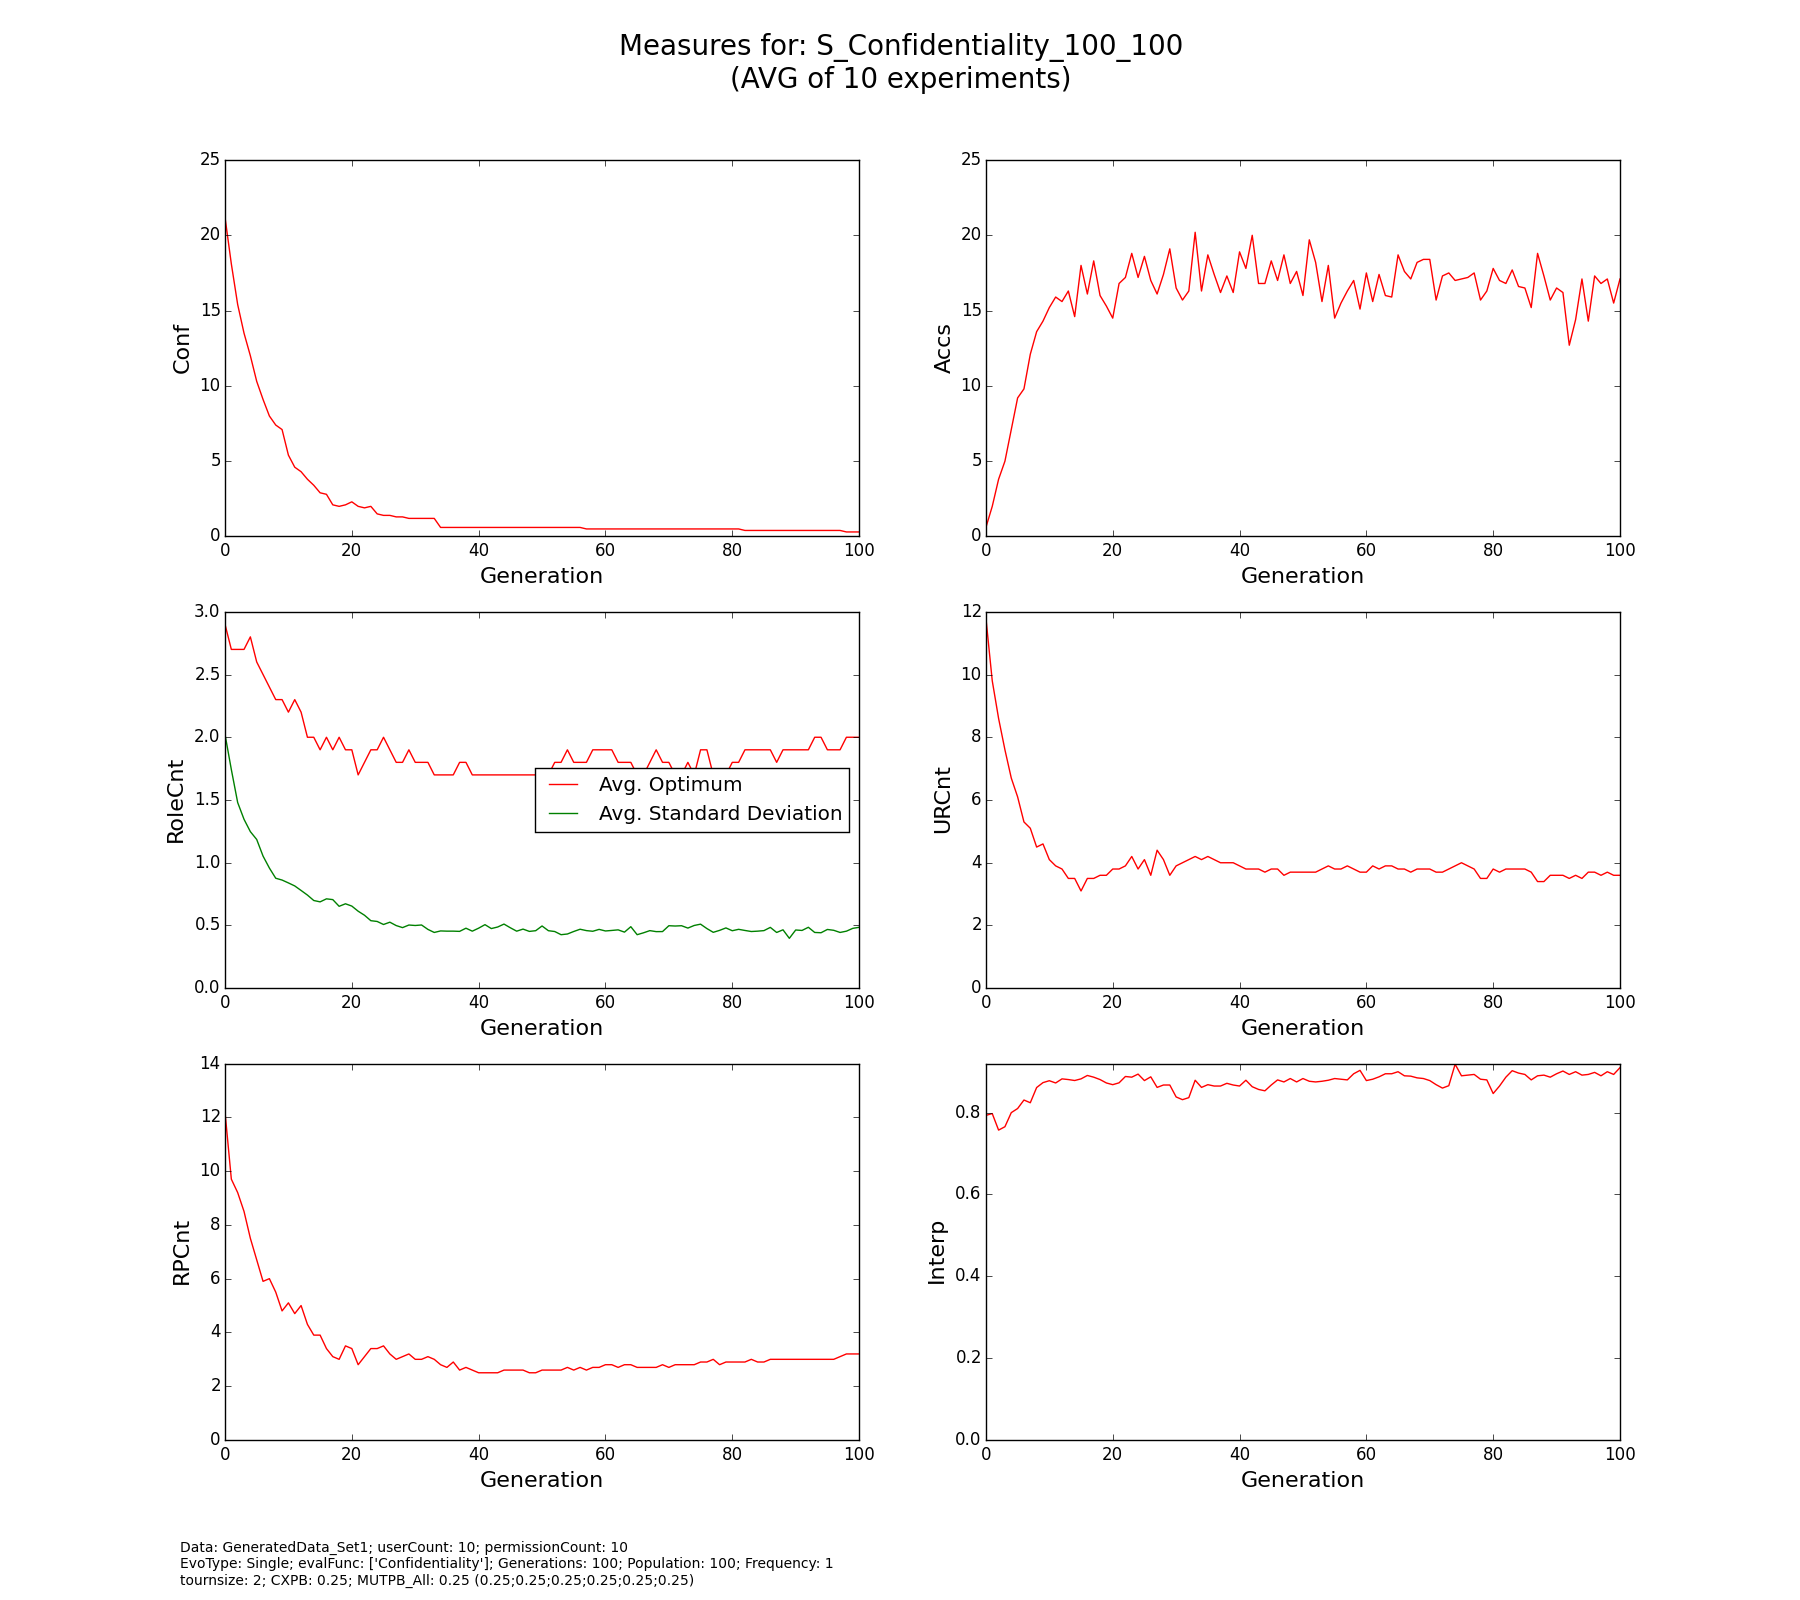
\includegraphics[scale=0.33, trim=4cm 2cm 4cm 0cm, clip=true]{exp1conf}
    \caption{EXPERIMENT 1a: Results of EvoRoleMiner with Fitness function $F=G_{conf}$ on synthetic dataset 1 with setup in table \ref{tab:setup1}. From u.l. to l.r.: Confidentiality Violations, Availability Violations, Role Count, User-Role Assignments, Role-Permission Assignments, Interpretability.}
    \label{fig:exp1conf}
\end{figure}

\begin{figure}[H]
    \centering
    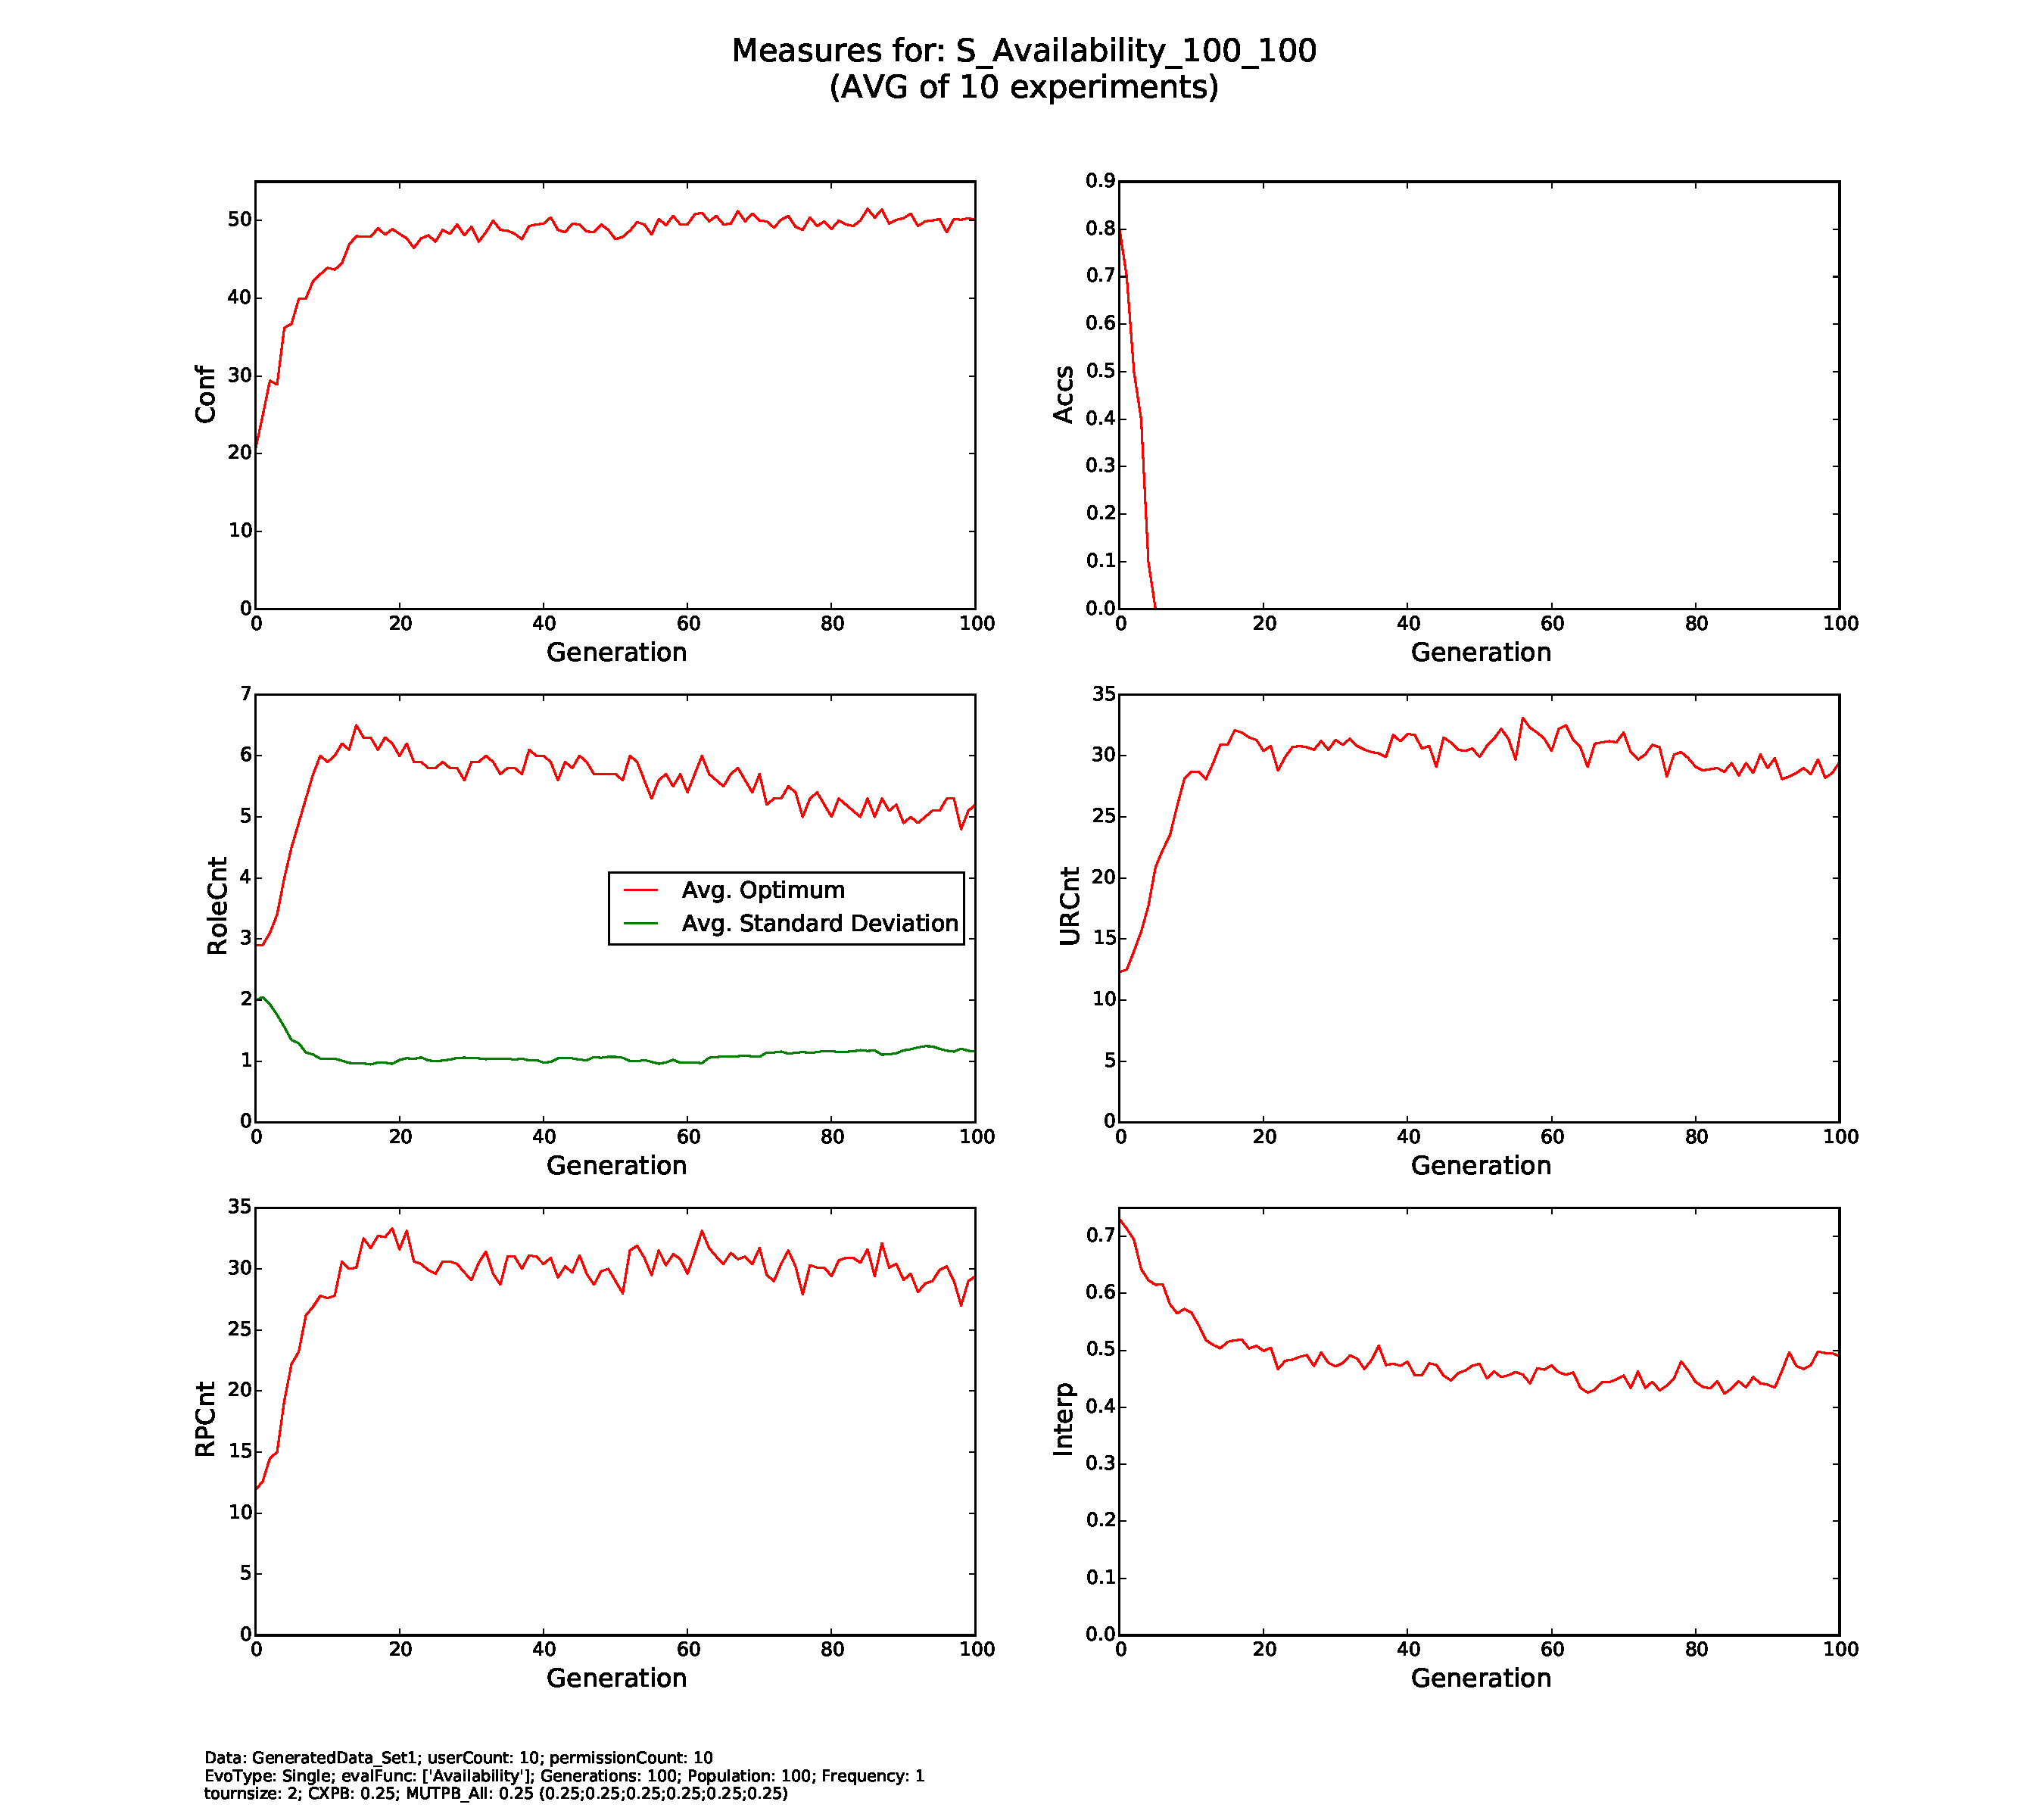
\includegraphics[scale=0.33, trim=4cm 2cm 4cm 0cm, clip=true]{exp1accs}
    \caption{EXPERIMENT 1b: Results of EvoRoleMiner with Fitness function $F=G_{accs}$ on synthetic dataset 1 with setup in table \ref{tab:setup1}. From u.l. to l.r.: Confidentiality Violations, Availability Violations, Role Count, User-Role Assignments, Role-Permission Assignments, Interpretability.}
    \label{fig:exp1accs}
\end{figure}